\providecommand{\main}{..}
\documentclass[\main/master.tex]{subfiles}
\begin{document}
\chapter{methods and results}\label{chp:example-2}
\section{vacuum system}
As explaned before when in vacuum viscous friction could be neglected. The torsional pendulum is placed inside a vacuum chamber, so the rotation angle is measured at vacuum.  since chamber is made from stainless steel, it's (a second) faraday cage, protecting from magnetic noise caused by measurement detectors.
\par
Vacuum chamber was manufactured using CF technology. Allowing to achieve ultra high vacuum (UHV), which would degrade to medium vacuum when pump is off. Chamber build is two cylindrical tubes placed on each other so the pendulum is inside, with three view ports in front. Sides viewports are used by the PID system to damp noises, and have a light guide before them. Center viewport is in front of the mirror placed on the pendulum and used to measure the rotation angle. The chamber has a 5 way which is connected to the vacuum engine and gauge.
\par
The angle measurement is made after the vacuum engine is disconnected from chamber by a valve, so it would not add rotation noise.






\section{torsion pendulum system}
The angle of torsion is measured using a mirror connected in front of the pendulum.This mirror is a part of an optical interferometer with which the mirror tilt could bedetermined.In order to balance the pendulum so the mirror would not be tilted, beside the tiltof the gravity field. The center of mass needs to be adjusted. The center of mass isadjusted using a mass from the back, to balance the mirror weight.The longer the wire and the smaller the wire diameter - wire torsion coefficient issmaller. Small coefficient achieves a better angle response to the gravity field. On theother hand the Small coefficient is leading to a very long time period of the pendulum,which while integrating over time would lead to very long measurements time. Alsothe wire needs to be strong enough to hold the masses without been teared down.


\section{Modulated CW Laser}
\subsection{devices}









\subsection{Laser}
The laser is a high power coherent light source based on stimulated emmission with narrow spectrum. Inside a cavity Electron is excited to a higher energy level, and forced by photon with the correct wavelength to be absorbed emmiting coherent photon. The coherence allows focusing to a tight spot, and the spot staying collimated over long distances. Continuous wave (CW) laser are lasing constant output power over time.  
\par
Usually the power output is stable but has oscillations due to having several longitudinal modes causing nano second scale ossicilations, output power is steady when averaged over longer periods. Also, over long periods of time lasers have slight power oscillations due to temperture changes in the envirement.
%The laser diode cavity face is rectangular, because of fabrication constraints. The rectangular face is causing cylindrical aberration, which   

\subsection{Acousto Optic Modulator}
Acousto Optic Modulator (AOM), uses the acousto-optic effect to diffract and shift the frequency of light using RF waves. An oscillating electric signal drives a piezoelectric transducer to vibrate causing RF waves, the transducer attached to a material. This causes sound waves in the material, and periodic index modulation causing a Bragg grating. Incoming light scatters off the grating and due to Bragg diffraction comes at Bragg angle.
\begin{equation}
\theta_b = sin(\theta_b)\approx \frac{\lambda}{2n\Lambda} \label{eqn:energy-mass-equivalence-relation}
\end{equation} 
$\Lambda$ is the RF wavelength, $\lambda$ is the light source wavelength. 
\par
Since all parameters constant, modulation angle is constant, and possible modulation speed is nano seconds. Giving a stable fast modulation method for CW laser.



\subsection{Light Emitting Diode (LED)}
The light emitting diode (led) is a high power long lifetime light source semiconductor based. The led is emitting light when current flows through. Led could be modulated at up to 100MHz. The initial opening angle of a led source varies between 45 to 120 degrees. The emitted light is incoherent in width meaning it's hard to focus it to a point (not diffraction limited). The emitted light is incoherent in length causing wide band spectrum, although spectrum is sufficiently narrow to appear as a pure color to the human eye.
\par
The working principle is a semiconductor p-n junction with direct band gap. Meaning the lowest energy state above the band gap has the same momentum as the highest under the gap. In order to change energy state electron needs only to release energy equal to the band gap, which defines the wavelength $E_g = \frac{\hslash c}{\lambda}$. All possible energy gaps defines the spectrum, aproximatly gaussian around the wavelength. Forward voltage is applied causing electron injection and recombination with holes. The recombination is releasing energy in form of spontanious emmission photons. The modulation limitation is due to the electrons life time before recombination.
\par
The led power is proptional to the current flows through, Shockley diode equation for p-n junction defines the current relation to the diode voltage. In high enough values the power could be aproximated by liniar aproximation of the diode voltage.
\begin{equation}
P\propto e^{\frac{q}{kT}\cdot V_d}\label{eqn:energy-mass-equivalence-relation}
\end{equation}

\subsection{arduino}
Arduino is an open-source microcontroller board project used for building low cost and simple digital devices and circuits. Each microcontroller contains a microprocessor, controller, serial communication interface and is equipped with digital and analog input/output pins. The microcontrollers are controlled using C and C++ programming languages, and could be operated as stand alone or connected to the computer through serial communication. 
\par
There are multiple Arduino board models, we would focus on Arduino Mega 2560. The Arduino Mega 2560 is based on the ATmega2560, an Atmel 8-bit AVR controller. Also the board has 54 digital input/output pins of which 15 could be used as PWM outputs and a 16 MHz crystal oscillator (clock). In reality the arduino doesn't have analog output, to modulate the output Pulse Width Modulation technique is used.
\par
The controller is switching on/off the signal between the full Vcc of the board and off (5-0[V]), generating a square wave. The duration of time signal on is called the pulse width. The controller is able to modulate the pulse width, and change the ratio of time signal is on compare to off. The voltage is determined by the ratio of the time voltage is on compare to time voltage off, which is called duty cycle. 100\% duty cycle means the power is always on, 0\% duty cycle power is always off and 50\% duty cycle signal is on and off in equal times. 
%\\
\par

\begin{figure}[htbp]
	\centering
	\fbox{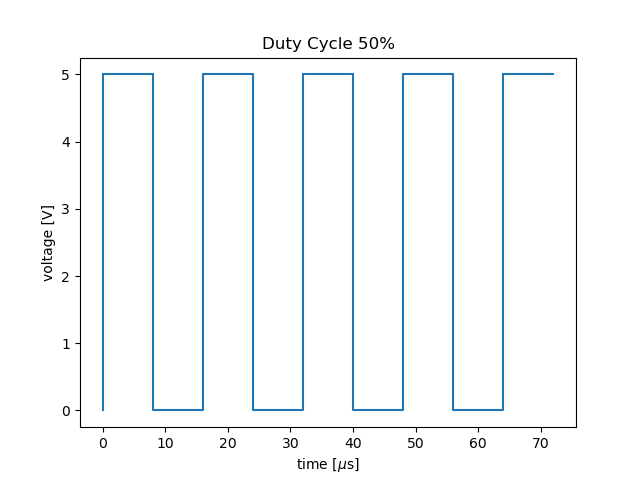
\includegraphics[scale=0.5]{\main/images/devices/duty50.png}}
	\caption[duty cycle 50\%]{50\% duty cycle  - signal is on and off equal times}
	\label{fig:duty50}
\end{figure}
Repeating that pattern fast enough results in an analog signal as if the signal is a steady voltage. This method is able to generate signals between the full Vcc of the board and off. The signal resolution is limited by the microcontroller resolution (8-bit). Due to the fast clock the of the arduino - the PWM analog modulation frequency is about 500Hz.
\par
\begin{figure}[htbp]
	\centering
	\fbox{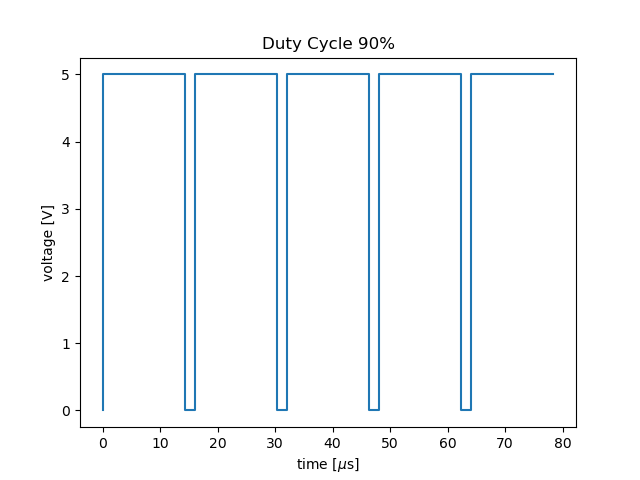
\includegraphics[scale=0.5]{\main/images/devices/duty90.png}}
	\caption[duty cycle 90\%]{90\% of the time signal on, equivalamt to 90\% of the full Vcc signal}
	\label{fig:duty90}
\end{figure}


\par
Using this method with a led connected, the led brightness could be modulated at about 2ms speed. Since the clock is connected to all PWM pins, if they all are in the same duty cycle, they are in sync. All pins are having a changing voltage, but they all have the same voltage, alowing to connect them in series and increase the output current, and the LED power. In conclusion this is a real-time controlled, fast-modulated, high power light source. 



\subsection{Light guides}
Light guides are pipes used for directed transmission of luminous energy.They are used to distribute light from the source to distant areas, they are made of thin filaments causing internal reflections. Light guides are used to illuminate small areas, regardless of the spectral characteristics of the light source. They mainly depend on the cross sections of entrance and exit and the length. Making them ideal to overcoming focusing problems, such as the LED uncoherent profile and large opening angle. 







\section{pid operate (algoritm)}
\section{laser +aom}
\section{laser +aom +amp}
\section{arduino + led}
\doublespacing
\hspace{5 mm} This another example chapter with a working reference as see in Chapter~\ref{chp:example-1}. There I also made an example of an equation, see Eqn.~\ref{eqn:energy-mass-equivalence-relation}. We also created an example image, see Fig.~\ref{fig:sine-wave}.
\begin{figure}[htbp]
	\centering
	\fbox{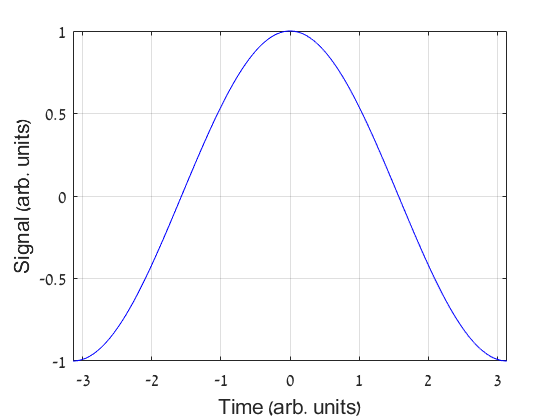
\includegraphics[scale=0.75]{\main/images/chapter_2_example/img_example_2.png}}
	\caption[Another Example Image]{Another Example Image. This image is also labeled internally so we can referenc it throughout the text.}
	\label{fig:cosine-wave}
\end{figure}
\end{document}